% topic_10.tex — Content only. Compiled via main.tex.
% ── No \documentclass, \begin{document} or \end{document} here ──

\chapteropener{10}{D.C. Circuits}{%
  \item Practical Circuits and E.M.F.
  \item Internal Resistance
  \item Kirchhoff's Laws
  \item Resistors in Series and Parallel
  \item Potential Dividers
  \item Thermistors and LDRs in Potential Dividers
}

% ===== SECTION 1: PRACTICAL CIRCUITS AND EMF =====
\section{Practical Circuits and E.M.F.}

\begin{definitionbox}{Electromotive Force (E.M.F.)}
The \textbf{electromotive force} (e.m.f., symbol $\varepsilon$) of a source is defined as the \textbf{energy transferred per unit charge} in driving charge around a complete circuit.
$$\varepsilon = \frac{W}{Q}$$
\begin{itemize}[itemsep=2pt]
  \item $W$: work done by the source (J); \quad $Q$: charge (C).
  \item Unit: volt (V) $\equiv$ J C$^{-1}$.
  \item E.m.f. is a \textbf{property of the source}; it represents energy input per coulomb.
\end{itemize}
\end{definitionbox}

\begin{definitionbox}{Potential Difference (P.D.)}
The \textbf{potential difference} (p.d.) between two points is the \textbf{energy transferred per unit charge} by a component as charge passes between those points.
$$V = \frac{W}{Q}$$
\begin{itemize}[itemsep=2pt]
  \item P.d. describes \textbf{energy released} (e.g.\ by a resistor); e.m.f. describes \textbf{energy supplied} (by a source).
  \item Both have unit: volt (V).
\end{itemize}
\end{definitionbox}

\begin{keybox}{E.M.F. vs P.D. — Energy Perspective}
\begin{itemize}[itemsep=2pt]
  \item \textbf{E.m.f.}: energy is \emph{given to} each coulomb of charge by the source (chemical $\to$ electrical).
  \item \textbf{P.d.}: energy is \emph{taken from} each coulomb of charge by a component (electrical $\to$ heat, light, etc.).
  \item Around any complete circuit: total e.m.f. = total p.d. (conservation of energy — see Kirchhoff's Second Law).
\end{itemize}
\end{keybox}

% ===== SECTION 2: INTERNAL RESISTANCE =====
\section{Internal Resistance}

\begin{definitionbox}{Internal Resistance}
A real source of e.m.f.\ has \textbf{internal resistance} $r$ — resistance within the source itself (e.g.\ chemical paste in a battery). As current flows, some energy is dissipated internally.
\end{definitionbox}

\begin{formulabox}{Terminal P.D. and Internal Resistance}
\begin{center}
\Large $\varepsilon = V + Ir \qquad \Longrightarrow \qquad V = \varepsilon - Ir$
\end{center}
\vspace{0.3em}
\begin{itemize}[itemsep=2pt]
  \item $V = \varepsilon - Ir$: \textbf{terminal p.d.} (voltage across the external circuit).
  \item $Ir$: \textbf{lost volts} — p.d.\ across internal resistance.
  \item $V < \varepsilon$ whenever current flows.
  \item For an external resistance $R$: $\displaystyle I = \frac{\varepsilon}{R + r}$
\end{itemize}
\end{formulabox}

\subsubsection*{Circuit diagram for a source with internal resistance}

\begin{center}
\begin{circuitikz}[european resistors, scale=1.1, every node/.style={font=\small}]
  % Battery with internal resistance
  \draw (0,0) -- (0,3) to[battery1, l=$\mathcal{E}$] (1.7,3)
              to[R, resistors/scale=0.7, l=$r$] (2.7,3)
              -- (4,3) -- (4,0)
              to[R, l=$R$] (0,0)
              ;
  % Dashed box around source
  \draw[dashed, darkgray, rounded corners] (0.4,2.5) rectangle (3,3.5);
  \node[darkgray, font=\footnotesize] at (1.1,2.2) {source};
  % Labels
  \node[midblue, font=\small] at (2,.6) {$V$};
  \draw[midblue, <->] (.2,0.4) -- (3.8,0.4);
\end{circuitikz}
\end{center}

\begin{warningbox}{Common Mistake}
The e.m.f.\ is \emph{not} the same as the terminal p.d.\ except when $I = 0$ (open circuit). Under load, $V = \varepsilon - Ir < \varepsilon$. Always check whether the question gives e.m.f.\ or terminal voltage.
\end{warningbox}

\subsubsection*{Graphical determination of $\varepsilon$ and $r$}

Rearranging: $V = \varepsilon - Ir$ has the form $y = c - mx$.

\begin{center}
\begin{tikzpicture}[xscale=2.8, yscale=2.2]
  % Axes
  \draw[->, darkblue, thick] (-0.1,0) -- (1.5,0) node[anchor=north, font=\small] {$I$};
  \draw[->, darkblue, thick] (0,-0.1) -- (0,1.3) node[anchor=east, font=\small] {$V$};
  % Line: V = 1.1 - 0.7*I
  \draw[midblue, thick] (0,1.1) -- (1.4, 0.13);
  % Intercept markers
  \draw[dashed, darkgray] (0,1.1) node[anchor=east, font=\small] {$\varepsilon$} -- (0.15,1.1);
  % Gradient annotation
  \draw[dashed, darkgray] (0.4, 0.82)  -- (0.4,0.33) -- (1.1,0.33);
  \node[darkgray, font=\footnotesize] at (0.7, 0.22) {$\Delta I$};
  \node[darkgray, font=\footnotesize] at (0.25, 0.52) {$\Delta V$};
  \node[pinkframe, font=\small, anchor=west] at (0.65, 0.8) {gradient $= -r$};
\end{tikzpicture}
\end{center}

\begin{itemize}[itemsep=2pt]
  \item \textbf{$y$-intercept}: $V = \varepsilon$ (e.m.f.\ when $I = 0$, i.e.\ open circuit).
  \item \textbf{Gradient}: $-r$ (magnitude of gradient gives internal resistance).
  \item \textbf{$x$-intercept}: $I = \varepsilon/r$ (short-circuit current; never reached safely).
\end{itemize}

% ===== SECTION 3: KIRCHHOFF'S LAWS =====
\section{Kirchhoff's Laws}

\vspace{2em}

\begin{definitionbox}{Kirchhoff's First Law (KCL)}
The sum of currents \textbf{entering} a junction equals the sum of currents \textbf{leaving} that junction.
$$\sum I_{\text{in}} = \sum I_{\text{out}}$$
This is a consequence of \textbf{conservation of charge} — charge does not accumulate at a junction.
\end{definitionbox}

\vspace{2em}

\begin{definitionbox}{Kirchhoff's Second Law (KVL)}
The sum of the e.m.f.s around any \textbf{closed loop} equals the sum of the potential differences (i.e.\ $IR$ products) around that loop.
$$\sum \mathcal{E} = \sum IR$$
This is a consequence of \textbf{conservation of energy} — a charge returning to its starting point has the same potential energy.
\end{definitionbox}

\vspace{2em}


\begin{keybox}{Sign Convention for Kirchhoff's Second Law}
\begin{itemize}[itemsep=2pt]
  \item Choose a direction to traverse the loop.
  \item \textbf{E.m.f.}: positive if traversed from $-$ to $+$ terminal (source adds energy); negative if $+$ to $-$.
  \item \textbf{$IR$}: positive if traversed in the same direction as current; negative if opposite.
  \item Apply consistently — the choice of direction does not affect the final answer.
\end{itemize}
\end{keybox}


\pagebreak

% Kirchoff's Law diagram

\subsubsection*{Circuit Diagram to show Kirchoff's Laws }

\tikzstyle{loop label}=[pinkframe,fill=white,scale=.8,inner sep=1]
\begin{center}
\begin{tikzpicture}[european resistors, scale=1.8]
  \draw[->,rounded corners=12,loop,pinkframe] (0.3,0.3) |- (3.7,2.8) |- (0.4,0.2);
  \draw[->,rounded corners=10,loop,pinkframe] (0.5,0.6) |- (1.7,2.6) |- (0.6,0.4);
  \draw[->,rounded corners=10,loop,pinkframe] (2.3,0.6) |- (3.5,2.6) |- (2.4,0.4);
  \draw (0,0) to[battery1,invert, l=$\mathcal{E}$] (0,1)
              to[R, resistors/scale=0.7, l=$r$] (0,1.45)
              -- (0,3) coordinate (I0) --++ (2,0) coordinate (I1)
              to[R,l=$R_1$] (2,0) coordinate (IF) -- (0,0);
  \draw (2,3) --++ (2,0) coordinate (I2)
              to[R,l=$R_2$] (4,0) -- (0,0);
  \node at (-0.35,0.22) {$-$};
  \node at (-0.35,0.80) {$+$};
  \draw[->,midblue] (I0)++(0.5, 0.1) --++ (1,0) node[midway,above] {$I_0$};
  \draw[->,midblue] (I1)++(0.1,-0.1) --++ (0,-0.65) node[midway,right,fill = white] {$I_1$};
  \draw[->,midblue] (I1)++(0.5, 0.1) --++ (1,0) node[midway,above] {$I_2$};
  \draw[->,midblue] (I2)++(0.1,-0.1) --++ (0,-0.65) node[midway,right] {$I_2$};
  \draw[->,midblue] (IF)++(-0.5,-0.1) --++ (-1,0) node[midway,below] {$I_0$};
  \node[loop label] at (0.90,2.78) {$c$};
  \node[loop label] at (1.12,2.62) {$a$};
  \node[loop label] at (2.92,2.62) {$b$};
\end{tikzpicture}
\end{center}


\begin{definitionbox}{Kirchoff's Closed Loops}
There are three \textbf{closed loops} shown in the diagram above, \textbf{a,b} and \textbf{c}.
\\
For \textbf{a} 
\begin{center}
$\mathcal{E}= I_{0}r + I_{1}R_{1}$

\end{center}


For \textbf{b} 
\begin{center}
$0= -I_{1}R_{1} + I_{2}R_{2}$

\end{center}

For \textbf{c} 
\begin{center}
$\mathcal{E}= I_{0}r + I_{2}R_{2}$

\end{center}

Also from Kirchoff's first law we know

\begin{center}
$I_{0} =I_{1}+I_{2}$

\end{center}
\end{definitionbox}

% ===== SECTION 4: RESISTORS IN SERIES AND PARALLEL =====
\section{Resistors in Series and Parallel}

\begin{formulabox}{Series Combination}
For $n$ resistors in series, the \textbf{same current} flows through each.
\begin{center}
\Large $R_{\text{total}} = R_1 + R_2 + R_3 + \cdots + R_n$
\end{center}
\vspace{0.2em}
\textit{Derivation (KVL):} $V = V_1 + V_2 + \cdots$; since $I$ is the same, $IR = IR_1 + IR_2 + \cdots$, hence $R = R_1 + R_2 + \cdots$
\end{formulabox}

\begin{center}
% Series diagram
\begin{circuitikz}[european resistors, scale=1.0, every node/.style={font=\small}]
  \draw (0,2) -- (0.3,2) to[R, l=$R_1$] (2.0,2) to[R, l=$R_2$] (3.7,2)
    to[R, l=$R_3$] (5.4,2) -- (5.7,2)
    -- (5.7,0) -- (0,0) to[battery1, l=$\varepsilon$, invert, i^>=$I$] (0,2);
  \node[darkblue, font=\small\bfseries] at (2.85, -0.5) {Series circuit — same $I$ throughout};
\end{circuitikz}

\vspace{1.5em}

\begin{formulabox}{Parallel Combination}
For $n$ resistors in parallel, the \textbf{same p.d.} exists across each.
\begin{center}
\Large $\frac{1}{R_{\text{total}}} = \frac{1}{R_1} + \frac{1}{R_2} + \frac{1}{R_3} + \cdots + \frac{1}{R_n}$
\end{center}
\vspace{0.2em}
\textit{Derivation (KCL):} $I = I_1 + I_2 + \cdots$; since $V$ is the same, $V/R = V/R_1 + V/R_2 + \cdots$, hence $1/R = 1/R_1 + 1/R_2 + \cdots$
\vspace{0.4em}

\textit{Special case for two resistors in parallel:}
$$R_{\text{total}} = \frac{R_1 R_2}{R_1 + R_2}$$
\end{formulabox}



% Parallel diagram
\begin{circuitikz}[european resistors, scale=1.0, every node/.style={font=\small}]
  \draw (0,3) -- (1,3);
  \draw (1,3) -- (1,4) to[R, l=$R_1$, i_<=$I_1$] (4,4) -- (4,3);
  \draw (1,3) -- (1,3) to[R, l=$R_2$, i_<=$I_2$] (4,3);
  \draw (1,3) -- (1,2) to[R, l_=$R_3$, i_<=$I_3$] (4,2) -- (4,3);
  \draw (4,3) -- (5,3) to[battery1, l_=$\varepsilon$, i=$I$] (5,0) -- (0,0) -- (0,3);
  \node[darkblue, font=\small\bfseries] at (2.5, -0.5) {Parallel circuit — same $V$ across each};
\end{circuitikz}
\end{center}

\begin{warningbox}{Common Mistake}
For two resistors in parallel, $R_{\text{total}}$ is \emph{always less} than the smaller of the two. If your answer is larger than either resistor, recheck your arithmetic — a common error is adding reciprocals incorrectly.
\end{warningbox}



% ===== SECTION 5: POTENTIAL DIVIDERS =====
\section{Potential Dividers}

\begin{definitionbox}{Potential Divider Principle}
A \textbf{potential divider} uses two (or more) resistors in series across a supply to produce a fraction of the supply voltage as an output.
$$V_{\text{out}} = V_{\text{in}} \times \frac{R_2}{R_1 + R_2}$$
\begin{itemize}[itemsep=2pt]
  \item $V_{\text{out}}$ is taken across $R_2$.
  \item The ratio $R_2/(R_1+R_2)$ determines the fraction of $V_{\text{in}}$ that appears across $R_2$.
  \item No current is drawn from the output (ideal case, or high-resistance load).
\end{itemize}
\end{definitionbox}

\begin{center}
\begin{circuitikz}[european resistors, scale=1.1, every node/.style={font=\small}]
  % Vertical chain
  \draw (0,4) to[battery1, l_=$V_{\text{in}}$] (0,0);
  \draw (0,4) -- (2,4) to[R, l=$R_1$] (2,2)
    to[R, l=$R_2$, -*] (2,0) -- (0,0);
  % Output taps
  \draw (2,2) -- (3.5,2) node[anchor=west] {$+$};
  \draw (2,0) -- (3.5,0) node[anchor=west] {$-$};
  \draw[midblue, <->] (3.2,0.1) -- (3.2,1.9);
  \node[midblue, anchor=west] at (3.35, 1.0) {$V_{\text{out}}$};
  % Node dot
  \node[fill=black, circle, inner sep=1.5pt] at (2,0) {};
\end{circuitikz}
\end{center}

\begin{keybox}{Potentiometer as a Comparison Tool}
A \textbf{potentiometer} is a sliding-contact potential divider used to \textbf{compare} e.m.f.s or p.d.s precisely:
\begin{itemize}[itemsep=2pt]
  \item A uniform resistance wire carries a \textbf{driver current} from a stable supply.
  \item The p.d.\ across a length $l$ of the wire is proportional to $l$.
  \item At \textbf{balance} (null deflection on galvanometer), no current is drawn from the test source — so the measurement is unaffected by internal resistance.
  \item $\dfrac{\varepsilon_1}{\varepsilon_2} = \dfrac{l_1}{l_2}$ at their respective balance lengths.
\end{itemize}
\end{keybox}


\pagebreak


\begin{definitionbox}{Null Method}
A \textbf{null method} is a measurement technique in which the quantity being measured is compared against a known standard and the detector (e.g.\ galvanometer) is adjusted to read \textbf{zero}. Because no current flows at balance, the result is independent of any resistance in the measuring instrument.
\end{definitionbox}

\vspace{4em}


\subsubsection*{Circuit Diagram for a Null Method Measurement }

\begin{center}
\begin{circuitikz}[american, european resistors, scale=2, every node/.style={font=\small}]
  % Driver circuit: battery + Resistor
  \draw (0,3) to[battery1] (2,3) to [R,l=R] (5,3)-- (5,2);
 
  % Wire AB
  \draw[very thick, midblue] (0,2) -- (5,2);
  \node at (1,3.5) {$\mathcal{E}_{driver}$};
  \node[anchor=north] at (-0.2,2) {A};
  \node[anchor=north] at (5,2) {B};
  
  % Sliding contact at balance point J
  \coordinate (J) at (3.0, 2);
  %\draw[fill=darkgray] (J) circle (2pt);
  \node[anchor=north] at (2.8,2) {J};
  % Test source + galvanometer branch
 
    \draw  (0,3) -- (0,0) to [battery1, l=$\mathcal{E}_x$] (1,0) to  [rmeter] (3,0) -- (3.0,1.8);
  \draw [-latex] (2,-.16) -- (2,.19);
   \draw [-latex](3,1.8) -- (J);
  % Balance length label
  \draw[<->, pinkframe] (0, 2.15) -- (3.0, 2.15);
  \node[pinkframe, anchor=south] at (1.6, 2.1) {$l$};
\end{circuitikz}
\end{center}


\pagebreak

% ===== SECTION 6: THERMISTORS AND LDRs =====
\section{Thermistors and LDRs in Potential Dividers}

\begin{definitionbox}{Thermistor (NTC)}
A \textbf{thermistor} (negative temperature coefficient, NTC) is a resistor whose resistance \textbf{decreases} as temperature \textbf{increases}. It is used as a temperature sensor in potential divider circuits.
\end{definitionbox}

\begin{definitionbox}{Light-Dependent Resistor (LDR)}
An \textbf{LDR} has resistance that \textbf{decreases} as light intensity \textbf{increases}. It is used as a light sensor in potential divider circuits.
\end{definitionbox}

\begin{keybox}{Using Sensors in Potential Dividers}
For a potential divider with a thermistor ($R_T$) in series with a fixed resistor $R$, with output taken across $R$:
$$V_{\text{out}} = V_{\text{in}} \times \frac{R}{R_T + R}$$
\begin{itemize}[itemsep=2pt]
  \item \textbf{Temperature rises} $\Rightarrow$ $R_T$ decreases $\Rightarrow$ $V_{\text{out}}$ \textbf{increases}.
  \item \textbf{Temperature falls} $\Rightarrow$ $R_T$ increases $\Rightarrow$ $V_{\text{out}}$ \textbf{decreases}.
  \item Swap the positions of $R_T$ and $R$ to \textbf{invert} the response (output high when cold, low when hot).
\end{itemize}
The same logic applies to an LDR replacing $R_T$, with light intensity replacing temperature.
\end{keybox}

\vspace{5em}

\begin{center}
\begin{circuitikz}[european resistors, scale=1.1, every node/.style={font=\small}]
  % Left: output across fixed R (high when hot)
  \draw (0,4) -- (0,3.5) to[thermistor, l_=$R_T$] (0,2) to[R, l_=$R$, -*] (0,0);
  \draw (0,4) node[anchor=south]{$V_{\text{in}}$};
  \draw[midblue, <->] (0.5,0.1) -- (0.5,1.9);
  \node[midblue, anchor=west] at (0.6,1.0) {$V_{\text{out}}$};
  \draw (0,0) -- (0.5,0);
  \draw (0,2) -- (0.5,2);
  \node[darkblue, font=\footnotesize, anchor=north] at (0,-0.3) {$V_{\text{out}}$ high when hot};

  % Right: output across thermistor (high when cold)
  \draw (4,4) -- (4,3.5) to[R, l_=$R$] (4,2) to[thermistor, l_=$R_T$, -*] (4,0);
  \draw (4,4) node[anchor=south]{$V_{\text{in}}$};
  \draw[midblue, <->] (4.5,0.1) -- (4.5,1.9);
  \node[midblue, anchor=west] at (4.6,1.0) {$V_{\text{out}}$};
  \draw (4,0) -- (4.5,0);
  \draw (4,2) -- (4.5,2);
  \node[darkblue, font=\footnotesize, anchor=north] at (4,-0.3) {$V_{\text{out}}$ high when cold};
\end{circuitikz}
\end{center}


% ===== SECTION 7: CIRCUIT SYMBOLS =====
\section{Circuit Symbols (Section 6 Reference)}

The following symbols from CIE Section 6 are required for Topic 10 circuit diagrams.

\begin{center}
\renewcommand{\arraystretch}{1.8}
\begin{tabular}{@{} p{3.8cm} c p{3.8cm} c @{}}
\toprule
\textbf{Component} & \textbf{Symbol} & \textbf{Component} & \textbf{Symbol} \\
\midrule

% Cell
Cell &
\begin{circuitikz}[scale=0.8, baseline=-3pt]
  \draw (0,0) to[battery1] (1.4,0);
\end{circuitikz} &
% Fixed resistor — european box with short leads either side
Fixed resistor &
\begin{tikzpicture}[scale=1, baseline=-3pt]
  \draw (0,0) -- (0.35,0);
  \draw (1.25,0) -- (1.6,0);
  \draw (0.35,-0.18) rectangle (1.25,0.18);
\end{tikzpicture} \\

% Battery of cells
Battery of cells &
\begin{circuitikz}[scale=0.8, baseline=-3pt]
  \draw (0,0) to[battery] (1.4,0);
\end{circuitikz} &
% Variable resistor — box with diagonal arrow (arrowhead at top-right)
Variable resistor &
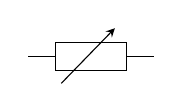
\begin{tikzpicture}[scale=1, baseline=-3pt]
  \draw (0,0) -- (0.35,0);
  \draw (1.25,0) -- (1.6,0);
  \draw (0.35,-0.18) rectangle (1.25,0.18);
  \draw[->, >=stealth] (0.42,-0.34) -- (1.1,0.36);
\end{tikzpicture} \\

% Switch — normally-open symbol: two lines with angled contact, no arrows
Switch &
\begin{circuitikz}[scale=0.8, baseline=-3pt]
  \draw (0,0) to[nos] (1.6,0);
\end{circuitikz} &
% Thermistor — box with plain diagonal line (no arrowhead)
Thermistor &
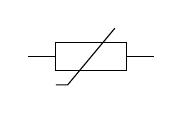
\begin{tikzpicture}[scale=1, baseline=-3pt]
  \draw (0,0) -- (0.35,0);
  \draw (1.25,0) -- (1.6,0);
  \draw (0.35,-0.18) rectangle (1.25,0.18);
  \draw (0.35,-0.36) -- (0.50,-0.36) -- (1.1,0.36);
\end{tikzpicture} \\

% Ammeter — circle with letter A, no diagonal arrow
Ammeter &
\begin{circuitikz}[scale=0.8, baseline=-3pt]
  \draw (0,0) to[rmeter, t=A] (1.6,0);
\end{circuitikz} &
% LDR — box with two bold diagonal arrows pointing toward box from upper-left
Light-dependent resistor &
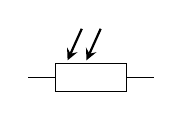
\begin{tikzpicture}[scale=1, baseline=-3pt]
  \draw (0,0) -- (0.35,0);
  \draw (1.25,0) -- (1.6,0);
  \draw (0.35,-0.18) rectangle (1.25,0.18);
  \draw[->, >=stealth, thick] (0.68,0.62) -- (0.50,0.22);
  \draw[->, >=stealth, thick] (0.92,0.62) -- (0.74,0.22);
\end{tikzpicture} \\

% Voltmeter — circle with letter V, no diagonal arrow
Voltmeter &
\begin{circuitikz}[scale=0.8, baseline=-3pt]
  \draw (0,0) to[rmeter, t=V] (1.6,0);
\end{circuitikz} &
% Galvanometer — circle with vertical upward arrow inside
Galvanometer &
\begin{circuitikz}[scale=0.8, baseline=-3pt]
  \draw (0,0) to[rmeter] (1.6,0);
  \draw [-latex] (0.8,-0.37) -- (0.8,0.4);
\end{circuitikz} \\

% Lamp
Lamp &
\begin{circuitikz}[scale=0.8, baseline=-3pt]
  \draw (0,0) to[lamp] (1.6,0);
\end{circuitikz} &
% Potentiometer — box with downward wiper arrow from top centre
Potentiometer &
\begin{tikzpicture}[scale=1, baseline=-3pt]
  \draw (0,0) -- (0.35,0);
  \draw (1.25,0) -- (1.6,0);
  \draw (0.35,-0.18) rectangle (1.25,0.18);
  \draw (0,0.42) -- (0.8,0.42);
  \draw[->, >=stealth] (0.8,0.42) -- (0.8,0.20);
\end{tikzpicture} \\

\bottomrule
\end{tabular}
\end{center}









% ===== SECTION 8: FORMULA SUMMARY =====
\section{Formula Summary Sheet}

\begin{minipage}{\linewidth}
\begin{tcolorbox}[colback=lightgold, colframe=accentgold]
\renewcommand{\arraystretch}{1.8}
\begin{tabular}{@{}lll@{}}
\toprule
\textbf{Formula} & \textbf{Quantity} & \textbf{Units} \\
\midrule
$\varepsilon = W/Q$ & E.m.f.\ definition & V \\
$V = \varepsilon - Ir$ & Terminal p.d. & V \\
$I = \varepsilon/(R + r)$ & Current in circuit & A \\
$R_{\text{total}} = R_1 + R_2 + \cdots$ & Series resistance & $\Omega$ \\
$1/R_{\text{total}} = 1/R_1 + 1/R_2 + \cdots$ & Parallel resistance & $\Omega$ \\
$R_{\text{total}} = R_1 R_2/(R_1+R_2)$ & Two resistors in parallel & $\Omega$ \\
$V_{\text{out}} = V_{\text{in}} \times R_2/(R_1+R_2)$ & Potential divider output & V \\
$\varepsilon_1/\varepsilon_2 = l_1/l_2$ & Potentiometer balance & — \\
\bottomrule
\end{tabular}
\end{tcolorbox}

\vspace{0.5em}
\begin{tcolorbox}[colback=lightblue, colframe=darkblue]
\textbf{KCL:}\quad $\sum I_{\text{in}} = \sum I_{\text{out}}$ at any junction (conservation of charge).\\[0.3em]
\textbf{KVL:}\quad $\sum \mathcal{E} = \sum IR$ around any closed loop (conservation of energy).\\[0.3em]
\textbf{Note:} Lost volts $= Ir$; terminal p.d.\ $< \mathcal{E}$ whenever current flows.
\end{tcolorbox}
\end{minipage}

% ===== SECTION 9: WORKED EXAMPLES =====
\section{Worked Examples}

\subsection*{Example 1 — Internal Resistance}

\textbf{Question:} A battery of e.m.f.\ $12\ \text{V}$ and internal resistance $0.5\ \Omega$ is connected to an external resistor of $3.5\ \Omega$. Calculate (a) the current, (b) the terminal p.d., and (c) the power dissipated internally.

\begin{examplebox}{Solution}
\textbf{(a)} \quad $I = \dfrac{\varepsilon}{R + r} = \dfrac{12}{3.5 + 0.5} = \dfrac{12}{4.0} = \mathbf{3.0\ \text{A}}$

\vspace{0.3em}
\textbf{(b)} \quad $V = \varepsilon - Ir = 12 - (3.0)(0.5) = 12 - 1.5 = \mathbf{10.5\ \text{V}}$

\vspace{0.3em}
\textbf{(c)} \quad $P_{\text{internal}} = I^2 r = (3.0)^2 \times 0.5 = 9 \times 0.5 = \mathbf{4.5\ \text{W}}$
\end{examplebox}

\subsection*{Example 2 — Kirchhoff's Laws}

\textbf{Question:} In the circuit below, $\varepsilon_1 = 10\ \text{V}$, $\varepsilon_2 = 4\ \text{V}$, $R_1 = 3\ \Omega$, $R_2 = 2\ \Omega$, $R_3 = 5\ \Omega$. Find the current flowing in the circuit (treat as a single loop, both sources driving in the same direction).

\begin{examplebox}{Solution}
Applying KVL around the loop (taking the direction of current as positive):
$$\sum \varepsilon = \sum IR$$
$$10 - 4 = I(3 + 2 + 5)$$
$$6 = 10I$$
$$I = \mathbf{0.60\ \text{A}}$$
\textit{Note}: if $\varepsilon_2$ had opposed $\varepsilon_1$, we would write $10 - 4$ on the left side (one e.m.f.\ is negative in our sign convention).
\end{examplebox}

\subsection*{Example 3 — Resistors in Parallel}

\textbf{Question:} Two resistors of $6\ \Omega$ and $12\ \Omega$ are connected in parallel across a $6\ \text{V}$ supply of negligible internal resistance. Find (a) the combined resistance, (b) the total current, and (c) the current through each resistor.

\begin{examplebox}{Solution}
\textbf{(a)} \quad $R_{\text{total}} = \dfrac{6 \times 12}{6 + 12} = \dfrac{72}{18} = \mathbf{4.0\ \Omega}$

\vspace{0.3em}
\textbf{(b)} \quad $I_{\text{total}} = V/R_{\text{total}} = 6/4.0 = \mathbf{1.5\ \text{A}}$

\vspace{0.3em}
\textbf{(c)} \quad $I_1 = 6/6 = \mathbf{1.0\ \text{A}}$;\quad $I_2 = 6/12 = \mathbf{0.50\ \text{A}}$

Check: $1.0 + 0.5 = 1.5\ \text{A}$ ✓ (KCL satisfied)
\end{examplebox}

\pagebreak

\subsection*{Example 4 — Potential Divider with Thermistor}

\textbf{Question:} A potential divider consists of a thermistor $R_T$ in series with a $1.5\ \text{k}\Omega$ fixed resistor, connected across a $5.0\ \text{V}$ supply. The output is taken across the fixed resistor. At $20\,^\circ\text{C}$ the thermistor has resistance $3.0\ \text{k}\Omega$. Calculate (a) $V_{\text{out}}$ at $20\,^\circ\text{C}$, and (b) whether $V_{\text{out}}$ increases or decreases as temperature rises.

\begin{examplebox}{Solution}
\textbf{(a)} \quad $V_{\text{out}} = 5.0 \times \dfrac{1500}{3000 + 1500} = 5.0 \times \dfrac{1500}{4500} = 5.0 \times \dfrac{1}{3} = \mathbf{1.67\ \text{V}}$

\vspace{0.3em}
\textbf{(b)} As temperature \textbf{rises}, $R_T$ \textbf{decreases}. The fraction $R/(R_T + R)$ \textbf{increases}, so $V_{\text{out}}$ \textbf{increases}.
\end{examplebox}


\pagebreak

% ===== SECTION 10: PRACTICE QUESTIONS =====
\section{Practice Exam Questions}

\subsection*{Section A — Short Answer Questions}

\begin{tcolorbox}[colback=white, colframe=midblue, breakable]

\begin{minipage}{\linewidth}
\textbf{Q1.} Define electromotive force (e.m.f.) and distinguish it from potential difference in terms of energy.
\par\hfill\textit{[3 marks]}
\vspace{3cm}
\end{minipage}

\begin{minipage}{\linewidth}
\textbf{Q2.} A cell has e.m.f.\ $9.0\ \text{V}$ and internal resistance $0.8\ \Omega$. When connected to a resistor, a current of $3.0\ \text{A}$ flows. Calculate (a) the terminal p.d.\ and (b) the power lost to internal resistance.
\par\hfill\textit{[3 marks]}
\vspace{3cm}
\end{minipage}

\begin{minipage}{\linewidth}
\textbf{Q3.} State Kirchhoff's first and second laws and give the physical principle underlying each.
\par\hfill\textit{[4 marks]}
\vspace{3.5cm}
\end{minipage}

\begin{minipage}{\linewidth}
\textbf{Q4.} Three resistors of $2\ \Omega$, $4\ \Omega$ and $6\ \Omega$ are connected in parallel. Calculate the combined resistance.
\par\hfill\textit{[2 marks]}
\vspace{2.5cm}
\end{minipage}

\end{tcolorbox}

\pagebreak

\subsection*{Section B — Longer Structured Questions}

\begin{tcolorbox}[colback=white, colframe=midblue, breakable]

\begin{minipage}{\linewidth}
\textbf{Q5.} A battery of e.m.f.\ $\varepsilon$ and internal resistance $r$ is connected to a variable external resistor $R$.
\end{minipage}

\begin{enumerate}[label=(\alph*)]
  \item \begin{minipage}[t]{\linewidth}
  Show that the terminal p.d.\ $V = \varepsilon - Ir$ and hence that $V = \varepsilon - \dfrac{\varepsilon r}{R+r}$.
  \par\hfill\textit{[2 marks]}
  \vspace{3cm}
  \end{minipage}

  \item \begin{minipage}[t]{\linewidth}
  A graph of $V$ against $I$ is plotted as $R$ is varied. Describe the graph and explain how $\varepsilon$ and $r$ can be determined from it.
  \par\hfill\textit{[3 marks]}
  \vspace{3.5cm}
  \end{minipage}

  \item \begin{minipage}[t]{\linewidth}
  Data from the graph gives $\varepsilon = 6.0\ \text{V}$ and $r = 0.4\ \Omega$. Calculate the current and terminal p.d.\ when $R = 2.6\ \Omega$.
  \par\hfill\textit{[3 marks]}
  \vspace{3cm}
  \end{minipage}
\end{enumerate}

\begin{minipage}{\linewidth}
\textbf{Q6.} The circuit shown consists of a supply of e.m.f.\ $12\ \text{V}$ and negligible internal resistance connected to resistors $R_1 = 4\ \Omega$, $R_2 = 6\ \Omega$ and $R_3 = 12\ \Omega$, where $R_2$ and $R_3$ are in parallel with each other and $R_1$ is in series with this parallel combination.

\begin{enumerate}[label=(\alph*)]
  \item Calculate the combined resistance of $R_2$ and $R_3$ in parallel.
  \par\hfill\textit{[2 marks]}
  \vspace{2.5cm}

  \item Calculate the total resistance of the circuit and the current drawn from the supply.
  \par\hfill\textit{[2 marks]}
  \vspace{2.5cm}

  \item Calculate the p.d.\ across the parallel combination and hence the current through each of $R_2$ and $R_3$.
  \par\hfill\textit{[3 marks]}
  \vspace{3.5cm}

  \item Verify your answers using Kirchhoff's first law.
  \par\hfill\textit{[1 mark]}
  \vspace{2cm}
\end{enumerate}
\end{minipage}

\begin{minipage}{\linewidth}
\textbf{Q7.} A potential divider consists of a $2.0\ \text{k}\Omega$ resistor and a light-dependent resistor (LDR) connected in series across a $10\ \text{V}$ supply. The output voltage is taken across the LDR. In bright light, the LDR has resistance $500\ \Omega$; in darkness, its resistance is $20\ \text{k}\Omega$.

\begin{enumerate}[label=(\alph*)]
  \item Calculate $V_{\text{out}}$ in bright light.
  \par\hfill\textit{[2 marks]}
  \vspace{2.5cm}

  \item Calculate $V_{\text{out}}$ in darkness.
  \par\hfill\textit{[2 marks]}
  \vspace{2.5cm}

  \item Explain how the circuit could be modified so that $V_{\text{out}}$ is high in bright light rather than in darkness.
  \par\hfill\textit{[1 mark]}
  \vspace{2.5cm}
\end{enumerate}
\end{minipage}

\end{tcolorbox}


\pagebreak

% ===== SECTION 11: MARK SCHEME =====
\section{Mark Scheme and Answers}

\begin{markscheme}

\textbf{Q1.} E.m.f.\ is the energy transferred \emph{to} each coulomb of charge by the source [1]; p.d.\ is the energy transferred \emph{from} each coulomb of charge by a component [1]; e.m.f.\ relates to energy input (e.g.\ chemical to electrical), p.d.\ relates to energy output (e.g.\ electrical to heat) [1].

\vspace{0.5em}\textbf{Q2(a).} $V = \varepsilon - Ir = 9.0 - (3.0)(0.8) = 9.0 - 2.4 = \mathbf{6.6\ \text{V}}$ [2].\\
\textbf{Q2(b).} $P = I^2 r = (3.0)^2 \times 0.8 = \mathbf{7.2\ \text{W}}$ [1].

\vspace{0.5em}\textbf{Q3.} KCL: sum of currents into a junction = sum of currents out [1]; consequence of conservation of charge [1]. KVL: sum of e.m.f.s around a closed loop = sum of $IR$ products [1]; consequence of conservation of energy [1].

\vspace{0.5em}\textbf{Q4.} $\dfrac{1}{R} = \dfrac{1}{2} + \dfrac{1}{4} + \dfrac{1}{6} = \dfrac{6+3+2}{12} = \dfrac{11}{12}$; \quad $R = \mathbf{12/11 \approx 1.1\ \Omega}$ [2].

\vspace{0.5em}\textbf{Q5(a).} By KVL: $\varepsilon = IR + Ir = I(R+r)$; rearranging gives $V = IR = \varepsilon - Ir$ [2].

\vspace{0.5em}\textbf{Q5(b).} Straight line [1]; $y$-intercept $= \varepsilon$ (open-circuit voltage) [1]; magnitude of gradient $= r$ [1].

\vspace{0.5em}\textbf{Q5(c).} $I = 6.0/(2.6+0.4) = 6.0/3.0 = \mathbf{2.0\ \text{A}}$ [1]; $V = 6.0 - (2.0)(0.4) = 6.0 - 0.8 = \mathbf{5.2\ \text{V}}$ [2].

\vspace{0.5em}\textbf{Q6(a).} $R_{23} = (6 \times 12)/(6+12) = 72/18 = \mathbf{4.0\ \Omega}$ [2].\\
\textbf{Q6(b).} $R_{\text{total}} = 4 + 4 = \mathbf{8.0\ \Omega}$; $I = 12/8 = \mathbf{1.5\ \text{A}}$ [2].\\
\textbf{Q6(c).} $V_{23} = 1.5 \times 4 = \mathbf{6.0\ \text{V}}$; $I_2 = 6/6 = \mathbf{1.0\ \text{A}}$; $I_3 = 6/12 = \mathbf{0.50\ \text{A}}$ [3].\\
\textbf{Q6(d).} $I_2 + I_3 = 1.0 + 0.5 = 1.5\ \text{A} = I_{\text{total}}$ ✓ [1].

\vspace{0.5em}\textbf{Q7(a).} $V_{\text{out}} = 10 \times 500/(2000+500) = 5000/2500 = \mathbf{2.0\ \text{V}}$ [2].\\
\textbf{Q7(b).} $V_{\text{out}} = 10 \times 20000/(2000+20000) = 200000/22000 = \mathbf{9.1\ \text{V}}$ [2].\\
\textbf{Q7(c).} Swap the positions of the LDR and the $2.0\ \text{k}\Omega$ resistor so that the output is taken across the fixed resistor instead [1].

\end{markscheme}

% ===== SECTION 12: REVISION CHECKLIST =====
\newpage
\section{Revision Checklist}

Use this checklist to track your understanding. Tick each box when you are confident:

\begin{tcolorbox}[colback=white, colframe=darkblue, breakable]
\renewcommand{\arraystretch}{1.5}
\begin{tabular}{@{} c p{10.5cm} r @{}}
\toprule
 & \textbf{Learning Objective} & \textbf{Confidence (1--3)} \\
\midrule
$\square$ & Recall and use the circuit symbols from Section 6 & \\
$\square$ & Define e.m.f.\ as energy transferred per unit charge by a source & \\
$\square$ & Distinguish between e.m.f.\ and p.d.\ in terms of energy & \\
$\square$ & Use \nf{V = \varepsilon - Ir} and \nf{I = \varepsilon/(R+r)} for circuits with internal resistance & \\
$\square$ & Determine $\varepsilon$ and $r$ from a $V$–$I$ graph (intercept and gradient) & \\
$\square$ & State and apply Kirchhoff's first law (conservation of charge) & \\
$\square$ & State and apply Kirchhoff's second law (conservation of energy) & \\
$\square$ & Derive and use \nf{R_{\text{total}} = R_1 + R_2 + \cdots} for series resistors & \\
$\square$ & Derive and use \nf{1/R_{\text{total}} = 1/R_1 + 1/R_2 + \cdots} for parallel resistors & \\
$\square$ & Use Kirchhoff's laws to solve multi-loop circuit problems & \\
$\square$ & Understand the principle of a potential divider circuit & \\
$\square$ & Use \nf{V_{\text{out}} = V_{\text{in}} \times R_2/(R_1+R_2)} for a potential divider & \\
$\square$ & Explain the potentiometer as a null method for comparing p.d.s & \\
$\square$ & Explain how a thermistor or LDR is used in a potential divider & \\
\bottomrule
\end{tabular}
\vspace{0.5em}

\textit{Key: 1 = Need more work \quad 2 = Getting there \quad 3 = Confident}
\end{tcolorbox}

\vspace{1em}
\begin{motivationbox}
\centering
\textbf{\color{darkblue}Good luck with your revision!}\\[0.2em]
{\color{darkgray}\small Kirchhoff's laws are nothing more than conservation of charge and conservation of energy written in circuit language. Once you see that, every circuit problem becomes a matter of careful bookkeeping — choose your loops, track your signs, and the algebra does the rest.}
\end{motivationbox}
